% Búsqueda local
La búsqueda local es un método heurístico para mejorar una dada solución factible a un problema. Se basa en, a partir de  una solución inicial $s$, mejorar esa solución iterativamente, tomando la mejor solución de un conjunto de vecinos de $s$. El conjunto de los vecinos se determina mediante algún criterio y se usa una función objetivo para comparar las soluciones en la vecindad de $s$ y discernir cual es la mejor.

La búsqueda local se puede expresar de la siguiente manera:\\\\
\hspace*{1 cm} Sea $s \in S$ una solución inicial\\
\hspace*{1 cm} Mientras exista $s' \in N(s)$ con $f(s') < f(s)$:\\
\hspace*{2 cm} $s \leftarrow s'$

Siendo $N(s)$ la vecindad de $s$ y $f$ la función objetivo que se quiere minimizar. Una versión de la búsqueda local se encarga además de que el vecino que elige minimice la función objetivo entre todas los vecinos.

% Solución inicial
\subsubsection{Solución inicial}

Como solución inicial se utilizó la heurística \texttt{Greedy} desarrollada en el punto anterior, consistente en elegir la mejor de tres corridas del algoritmo de Dijkstra con distintas funciones de peso.

% Definición de la vecindad
\subsubsection{Definición de la vecindad}

En cada iteración definimos la vecindad de $s$, $N(s)$, de la siguiente manera: dado el grafo G, y una solución formada por un camino $c \in G$, definimos sus soluciones vecinas como aquellas resultantes de tomar un subcamino $d_{n_1,n_2} \subseteq c$ entre un par de nodos $n_1,n_2$ cualesquiera, y reemplazarlo por otro camino $d_{n_1,n_2}^*$ en $G$, de tal forma que el camino $c^* = c - d_{n_1,n_2} + d_{n_1,n_2}^*$ resultante cumpla: 

\begin{itemize}
\item $\omega_1(c^*)$ $<=$ $K$
\item $\omega_2(c^*)$ $<$ $\omega_2(c)$
\item $c^*$ no contiene ciclos
\end{itemize}

De la forma descripta, dada una solución formada por un camino $c$ definimos su vecindad como el conjunto $S^*$ de todos los caminos $c^*$ posibles.

Corremos previamente $n$ veces Dijkstra, una vez desde cada nodo. Guardamos los resultados en una matriz tal que en la posición $[i][j]$ guarda el camino mínimo del nodo $i$ al $j$. Cada camino $d_{n_1,n_2}^*$ es el camino mínimo entre $n_1$ y $n_2$ según $\omega_2$, se obtiene de la matriz. Debe además cumplir $\omega_1(c^*) \leq K$. De todos los $c^*$, se elige el que minimice $\omega_2$. Esto se enmarca en la elección de vecinos utilizando el método \textit{Steepest Descent} consistente en elegir al vecino que minimice la función objetivo.

Puede darse el caso de que, al reemplazar un camino $d_{n_1,n_2}$ por $d_{n_1,n_2}^*$, existan nodos en este último que también existan en $c^* = c - d_{n_1,n_2}$, de tal forma que el camino $c^*$ resultante contenga ciclos. Para resolver este inconveniente, luego de efectuar cada reemplazo, se llama al método removeCycles, el cual toma un camino, ya sea con ciclos o sin ciclos, y se encarga de construir una versión del mismo la cual no contenga ciclos.

Ahora, para calcular $\omega_2(c^*)$, lo calculamos como

\[
\omega_2(c) - \omega_2(d_{n_1,n_2}) + \omega_2(d_{n_1,n_2}^*)
\]

, valores que ya tenemos calculados.

\subsubsection{Pseudocódigo}

El algoritmo está implementado en la función \texttt{main}:

\begin{algorithm}[H]
\caption{$main$(int tipo\_solucionInicial, Graph g, Nodo n1, Nodo n2)}
\begin{algorithmic}[1]
  \State crearMatrizCaminosMinimos(g)
  \State Solution solucion = \texttt{Greedy(g, n1, n2)}
  
  \If{$\omega_1$(solucion) $\leq$ K}    
    \While{True}    	        
    	\State Solution nuevaSolucion = dameMejorVecino(solucion)
	\If{nuevaSolucion == NULL} 
		\State break	
	\EndIf    
	\State solucion = nuevaSolucion	
    \EndWhile
  \EndIf
\end{algorithmic}
\end{algorithm}

\begin{algorithm}[H]
\caption{$dameMejorVecino$(Solution solucionOriginal)}
\begin{algorithmic}[1]	
          \State Solution mejorSolucion = \&solucionOriginal
	  \State vector$<int>$ nodos = \&nodos(solucionOriginal)
	  \For{i=0; i $<$ size(nodos); i++}
	  	\For{j=i+1; j $<$ size(nodos); j++}
			\State Solution subSolucion = crearSubSolucionEntre(solucionOriginal, nodos[i], nodos[j])
			\State Solution solucion\_ij = dameCaminoResueltoEntre(nodos[i], nodos[j])
                        \State removerCiclos(solucion\_ij)
			\State Solution nuevaSolucion\_$\omega_2$ = $\omega_2$(solucionOriginal) - $\omega_2$(subSolucion) + $\omega_2$(solucion\_ij)
			\State Solution nuevaSolucion\_$\omega_1$ = $\omega_1$(solucionOriginal) - $\omega_1$(subSolucion) + $\omega_1$(solucion\_ij)			
			\If{nuevaSolucion\_$\omega_2$ $<$ $\omega_2$(mejorSolucion) \&\& nuevaSolucion\_$\omega_1$ $\leq$ K)}
				\State mejorSolucion = crearSolucionReemplazandoCamino(solucionOriginal, solucion\_ij)
			\EndIf
		\EndFor
	\EndFor
	\State return mejorSolucion
\end{algorithmic}
\end{algorithm}

\begin{algorithm}[H]
\caption{$crearSolucionReemplazandoCamino$(Solution orig, Solution sub)}
\begin{algorithmic}[1]	
	 \State Solution res
	 \State res = obtenerCaminoHasta(nodos(sub)[0])
	 \State res += sub
	 \State int subSize = size(nodos(sub))
	 \State res += obtenerCaminoDesde(nodos(sub)[subSize-1])	  
	\State return res
\end{algorithmic}
\end{algorithm}

\begin{algorithm}[H]
\caption{$removerCiclos$(Solution solution)}
\begin{algorithmic}[1]	
	 \State int nextNodes[nodeCount]
	 \For{i=0; i $<$ nodeCount; i++}
	 	\State nextNodes[i] = 0
	\EndFor
	 \For{i=0; i $<$ solution.path.size(); i++}
		 \State edge = solution.path[i]
	 	\State nextNodes[edge.fromNode] = edge.toNode
	\EndFor	
	 \State vector$<int>$ newPath
	 \State firstNode = solution.path[0].fromNode
	 \State lastNode = solution.path[solution.path-1].toNode
	 \State next = firstNode
	 \State newPath.push(firstNode)
	 \While{nextNodes[next] != lastNode}
	 	\State next = nextNodes[next]
		\State newPath.push(next)
	\EndWhile
	\State newPath.push(lastNode)
	\State Solution newSolution
	\For{i=0; i $<$ newPath.size()-1; i++}	
		\State edge = solution.getEdgeBetween(newPath[i], newPath[i+1]
		\State newEdge = Edge(edge)
		\State newSolution.addEdge(edge)
	\EndFor
	\State return newSolution
\end{algorithmic}
\end{algorithm}

% Complejidad
\subsubsection{Complejidad}

Implementamos el algoritmo en la función $main$. La complejidad del algoritmo resulta la suma de obtener la solución inicial y el ciclo que se usa para mejorarla buscando un mejor vecino en cada iteración. 
Además, en $main$, inicialmente, se llama a una función crearMatrizCaminosMinimos\footnote{\label{$crearMatrixCaminosMinimos$}: Estamos haciendo uso de esta función que no se encuentra en el código fuente como tal, pero es para facilitar la legibilidad del pseudocódigo. En el código fuente se crea la matriz de camino mínimos cuando se inicializa NeighbourhoodSelector en la función main en localsearch.cpp.}, que abordaremos más adelante.

Creamos la solucion inicial usando Greedy. Esta función como explicamos en el apartado anterior, devuelve un camino mínimo entre 2 nodos usando Greedy A, B y C. Cada una de las 3 funciones Greedy usan la función resolverConDijkstra que ejecuta Dijkstra para encontrar todos los caminos mínimos entre n1 y los demás nodos y después hace un recorrido inverso desde n2 hasta n1 para dar con el camino mínimo entre ellos. Como se comprobó en el apartado anterior, la complejidad de Dijkstra es $O(m log(n))$ y el recorrido inverso es $O(n)$, por lo que en total la complejidad de obtenerSolucionInicial es $O(m log(n))$. Cabe notar que la función objetivo usada en Dijkstra no influye en la complejidad, ya que solo compara los valores de $\omega_1$ y $\omega_2$, por lo que tiene complejidad $O(1)$.

Para mejorar la solución usamos un ciclo y en cada iteración obtenemos el mejor vecino del camino actual usando dameMejorVecino. Ejecutamos el ciclo mientras en la última iteración hayamos encontrado una mejora al camino actual. 
Dado que un vecino consiste en reemplazar la porción del camino actual que une 2 nodos $n_1$ y $n_2$ por el camino mínimo según $\omega_2$ entre ellos, y que cada vez que se hace el reemplazo se disminuye $\omega_2$ del camino actual, se pueden hacer a lo sumo tantos reemplazos como caminos mínimos entre todo par de nodos del grafo existan. 
La cantidad de caminos mínimos entre todo par de nodos de un grafo es $n \times (n-1) / 2$, ya que cada nodo tiene un camino mínimo hacia todos los demás y no a sí mismo. Esto es, si hay n nodos, el nodo $n_1$, tiene un camino mínimo hacia los nodos $n_2$, ..., $n_n$, el nodo $n_2$ tiene un camino hacia $n_3$, ..., $n_n$ ya que no se vuelve a contar el camino entre $n_1$ y $n_2$ y así hasta $n_{n-1}$ que tiene un camino hasta $n_n$.
Luego, la cantidad máxima de iteraciones es $n \times (n-1) / 2$.

Para analizar la complejidad de cada iteración hay que analizar la complejidad de dameMejorVecino. 
Lo primero que hace la función es obtener el arreglo de nodos de la solución pasada por parámetro, que llamamos solucionOriginal. Cómo el camino de solucionOriginal está representado como una lista de ejes, lo que hace es iterar por todos los ejes y tomar el nodo1 del eje y al final adicionar el nodo2 del último eje. Por ende, tomando $t$ como la cantidad de nodos en el camino, en cada iteración, por cada eje del camino, se toma un nodo y esto se hace $t$-1 veces y luego se añade el nodo final. Como $t$ puede ser a lo sumo $n$, entonces la complejidad de esto resulta $O(n^2)$.
Luego de ejecuta un doble $for$ de $t \times (t-1) / 2$ iteraciones, que en cada iteración intenta mejorar el mejor camino encontrado hasta el momento, que llamamos mejorSolucion. Inicialmente mejorSolucion es igual a solucionOriginal. 
Para encontrar una mejor solución en cada iteración hacemos lo siguiente:

\begin{itemize}
\item Creamos el subcamino de solucionOriginal entre los nodos $n_1$ y $n_2$.
\item Obtenemos el camino mínimo entre los nodos $n_1$ y $n_2$.
\item Obtenemos un nuevo camino reemplazando el el subcamino entre los nodos $n_1$ y $n_2$ por el camino mínimo entre ellos.
\end{itemize}

Para crear el subcamino de solucionOriginal entre $n_1$ y $n_2$ usamos crearSubSolucionEntre. Esta función recibe un par de nodos y un camino y devuelve el subcamino que une a los nodos. Para esto tiene que recorrer a lo sumo todos los nodos del camino, o sea $t$, que puede ser a lo sumo $n$.

Para obtener el camino mínimo entre los nodos $n_1$ y $n_2$ usamos una optimización que es que en la función $main$, al comienzo, ejecutamos crearMatrizCaminosMinimos que crea una matriz de caminos mínimos entre todo par de nodos del grafo. Generamos esta matriz ejecutando Dijkstra para todos los nodos usando como función objetivo $\omega_2$. Usamos esta matriz para obtener en $O(1)$ el camino mínimo entre los nodos $n_1$ y $n_2$.
Como crearMatrizCaminosMinimos ejecuta un Dijkstra por cada nodo, su complejidad es $O(n \times (m log n))$.

Para obtener el nuevo camino reemplazando el subcamino entre $n_1$ y $n_2$ por el camino mínimo entre ellos, usamos crearSolucionReemplazandoCamino.
Lo que hacemos es generar una nueva solución que es la concatenación de 3 caminos: el camino mínimo entre $n_1$ y $n_2$ y los dos pedazos del camino original sin el subcamino que unía $n_1$ y $n_2$. Para crear el camino, hay que recorrer el solucionOriginal y añadir todos los nodos hasta $n_1$ y luego añadir todos los nodos del camino mínimo y al final añadir todos los nodos desde $n_2$ hasta el final de solucionOriginal. Por ende es como iterar sobre el nuevo camino que a lo sumo puede tener $n$ nodos y por ende la complejidad resulta $O(n)$.

Como es posible que la solución creada a partir de unir los caminos contenga ciclos, usamos la función removerCiclos que se encarga de remover cualquier ciclo en la nueva solución. Esta función itera sobre los nodos de la solución y almacena en un arreglo de enteros el nodo siguiente a cada nodo. De modo que cada elemento i corresponde al nodo i y su valor es el nodo siguiente a ese nodo i. En el caso de que exista un ciclo y un nodo i esta al comienzo de un ciclo, primero el nodo i tendrá como siguiente a otro nodo j, pero cuando se itera sobre la solución y se llega nuevamente al nodo i, al asignarle su siguiente, ese nodo ya no será j, sino otro nodo mas adelente en la solución. Con el arreglo creado de esa manera podemos reconstruir la solución sin ciclos. El camino se obtiene recorriendo el arreglo como una lista enlazada, donde cada elemento tiene el índice del siguiente. Usando este arreglo creamos una nueva solución, que es un vector de ejes con $omega_1$ y $omega_2$ asignados. Los ejes los construimos usando los nodos del arreglo y obtenemos los valores de $omega_1$ y $omega_2$ de la solución recibida por parametro. La complejidad de remover los ciclos resulta igual a la suma de construir el arreglo, que es $O(n)$, ya que a lo sumo puede tener n vertices y luego crear la nueva solución que es $O(n^2)$, ya que hay que crear hasta $n-1$ ejes y por cada eje hay que obtener sus valores de $omega_1$ y $omega_2$ de la solución original. Luego en total es $O(n^2)$. 

Entonces, resulta ser que encontrar el mejor vecino, consiste en ejecutar el doble $for$ de algo que tiene complejidad $O(n + 1 + n + n^2)$, o sea $O(n^2)$, entonces en total es $O(n^2 \times n^2) = O(n^4)$.

Como habíamos explicado que dameMejorVecino se ejecuta en un ciclo de hasta $n \times (n-1) / 2$ iteraciones, o sea $O(n^2)$, y entonces resulta que la complejidad de encontrar el mejor vecino es $O(n^2 \times n^4) = O(n^6)$. 

Finalmente la complejidad total resulta ser la suma de las complejidades de crearMatrizCaminosMinimos, 2 veces obtenerSolucionInicial y $n^2$ veces dameMejorVecino. Es decir, $O(n \times (m log n) + 2 \times (m log n) + n^6) = O(n^6)$.

% Familias malas
\subsubsection{Familias malas}

Veamos que nuestra heurística de búsqueda local puede quedar arbitrariamente lejos de la solución óptima.

Presentamos la siguiente familia de grafos:

\ponerGrafico{imagenes/maloLocalA.png}{}{0.5}{malo-para-local-a}

Para ir de 1 a 5 hay tres caminos posibles: ($C_1$) $1 \rightarrow 2 \rightarrow 5$; ($C_2$) $1 \rightarrow 3 \rightarrow 5$;
($C_3$) $1 \rightarrow 4 \rightarrow 5$;

\begin{eqnarray}
 \omega_1(C_1) &=& 4	\\ 
 \omega_2(C_1) &=& 2	\\
 \omega_1(C_2) &=& 2	\\
 \omega_2(C_2) &=& 2x   \\
 \omega_1(C_3) &=& 6	\\
 \omega_2(C_3) &=& 1
\end{eqnarray}

Supongamos que K vale 4.
Como decíamos, partimos del camino mínimo entre $u$ y $v$ de acuerdo a $\omega_1$, $C_2$. El algoritmo va a intentar intercambiar $C_2$ por
$C_3$, el camino que minimiza $\omega_2$. Sin embargo, como éste se pasa del límite K, el algoritmo no puede seguir y devuelve $C_2$. Sin
embargo $C_1$ era una solución mejor.

$\frac{\omega_2(C_2)}{\omega_2(C_1)} = x$.

Haciendo crecer el valor de $x$ podemos encontrar grafos en los que nuestro algoritmo devuelve una
solución arbitrariamente lejos de la óptima.

En general, la heurística falla cuando los caminos mínimos por $\omega_2$ entre todo par de nodos tienen un valor de $\omega_1$ demasiado alto, que deja a la solución sin vecinos factibles ya que éstos se sobrepasan de la restricción de $K$.
\newpage

\subsubsection{Experimentación}

Pudimos analizar el tiempo de ejecución corriendo el algoritmo en grafos de un tamaño considerable. Utilizamos instancias del tipo \textit{mágico}, variando el valor de $n$ y eligiendo $m$ al azar entre todos los posibles valores dado $n$.  A continuación presentamos un gráfico.

\begin{figure}[H]
\begin{center}
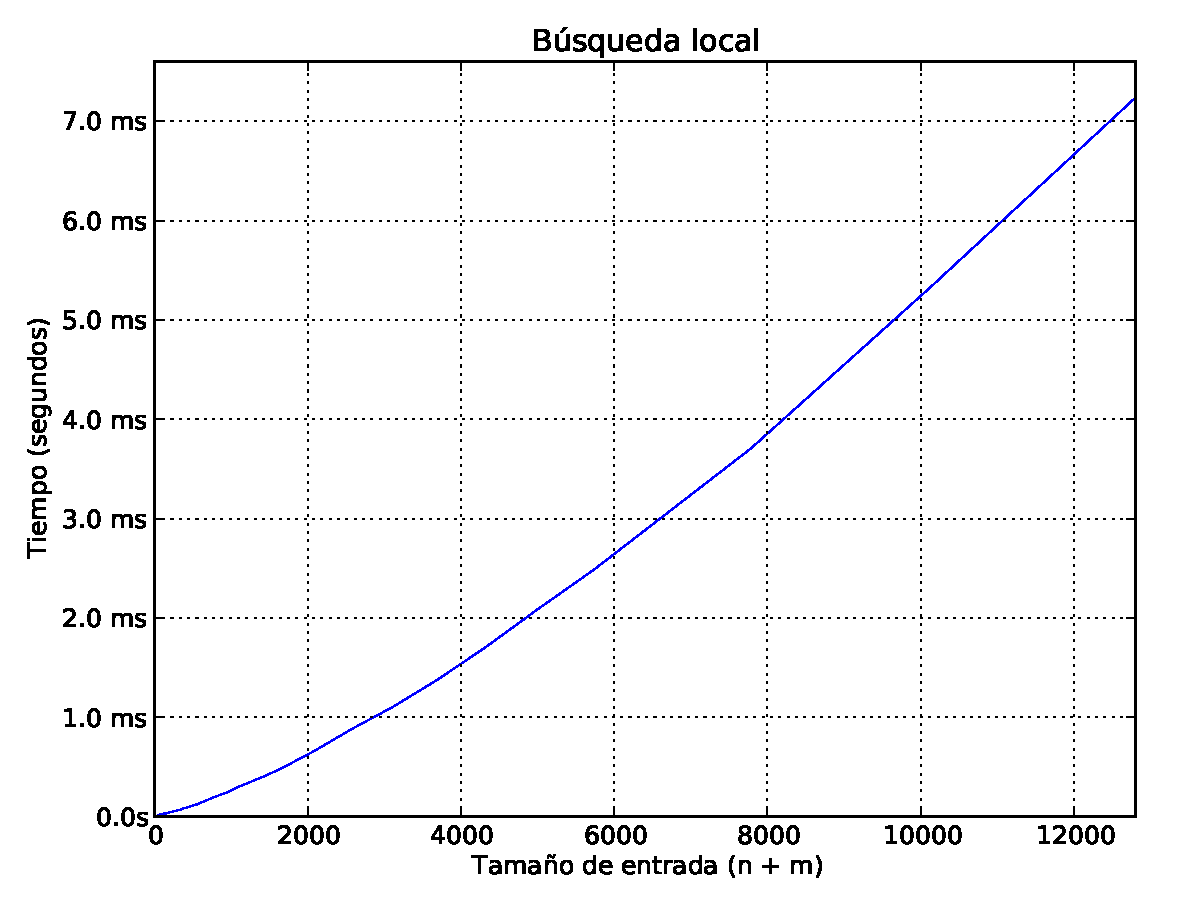
\includegraphics[angle=0, scale=.75]{imagenes/local_search_time.pdf}
\label{grafico local}
\end{center}
\end{figure}


Se puede percibir el carácter no lineal de la complejidad. Sin embargo no se evidencia a luces claras la cota teórica de $n^6$ desarrollada
previamente. Puede ser necesario un tamaño mayor para poder apreciar esa complejidad, o quizás la cota teórica no se alcanza en la práctica.
Probablemente haya un factor que se amortice, habiendo escapado de nuestro escrutinio.

La conclusión que se obtuvo tras haber terminado todas las experimentaciones es que \texttt{local\_search} hace generalmente pocas iteraciones, por lo que el tiempo de ejecución se asemeja al de \texttt{Greedy}, cuya complejidad teórica es $O(m*log(n)$.

\newpage
Luego se propuso analizar la calidad de la solución encontrada.
Experimentamos con distintas densidades de grafos. Primero con grafos densos, es decir con una cantidad de aristas del orden de $n^2$. Luego con
grafos de densidad media, con una cantidad de aristas del orden de $\sqrt{n} \times n$. Finalmente probamos con grafos ralos, con una cantidad de aristas
del orden de la cantidad de nodos. Para cada grupo de grafos, analizamos diferentes rangos de tamaños de entrada, con el objetivo de demostrar
que el algoritmo mantiene ciertas propiedades, más allá del tamaño.

Se generan cien instancias para cada tamaño de entrada. En los siguientes gráficos se pueden observar comparados el mejor resultado, el peor
resultado, y el resultado promedio para cada tamaño de entrada. Al ser instancias del tipo \textit{mágico}, podemos saber el valor de la solución óptima - $n-1$ - y graficarla.

\begin{figure}[H]
\begin{center}
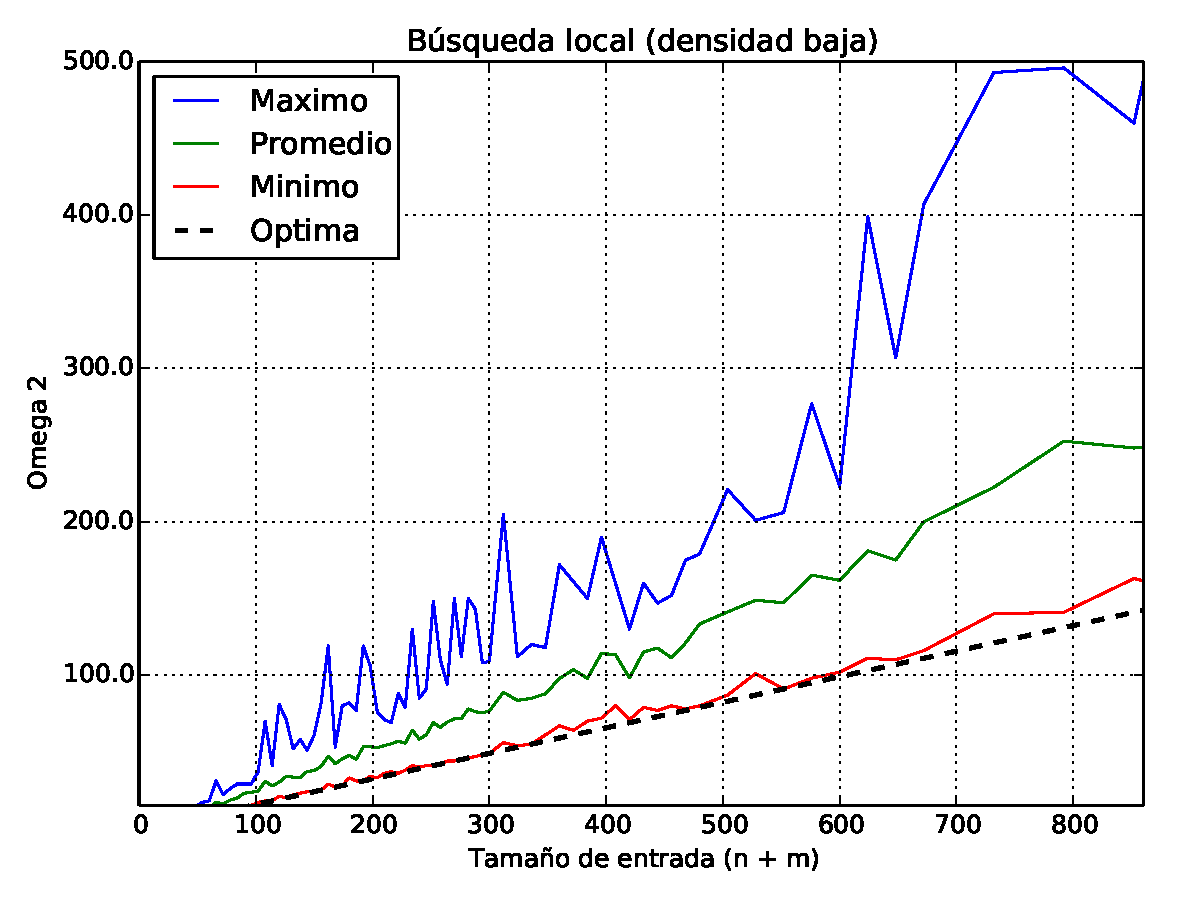
\includegraphics[angle=0, scale=.70]{imagenes/calidad_local_search_2014-06-27_16-02-57.pdf}
\label{grafico local}
\end{center}
\end{figure}

\begin{figure}[H]
\begin{center}
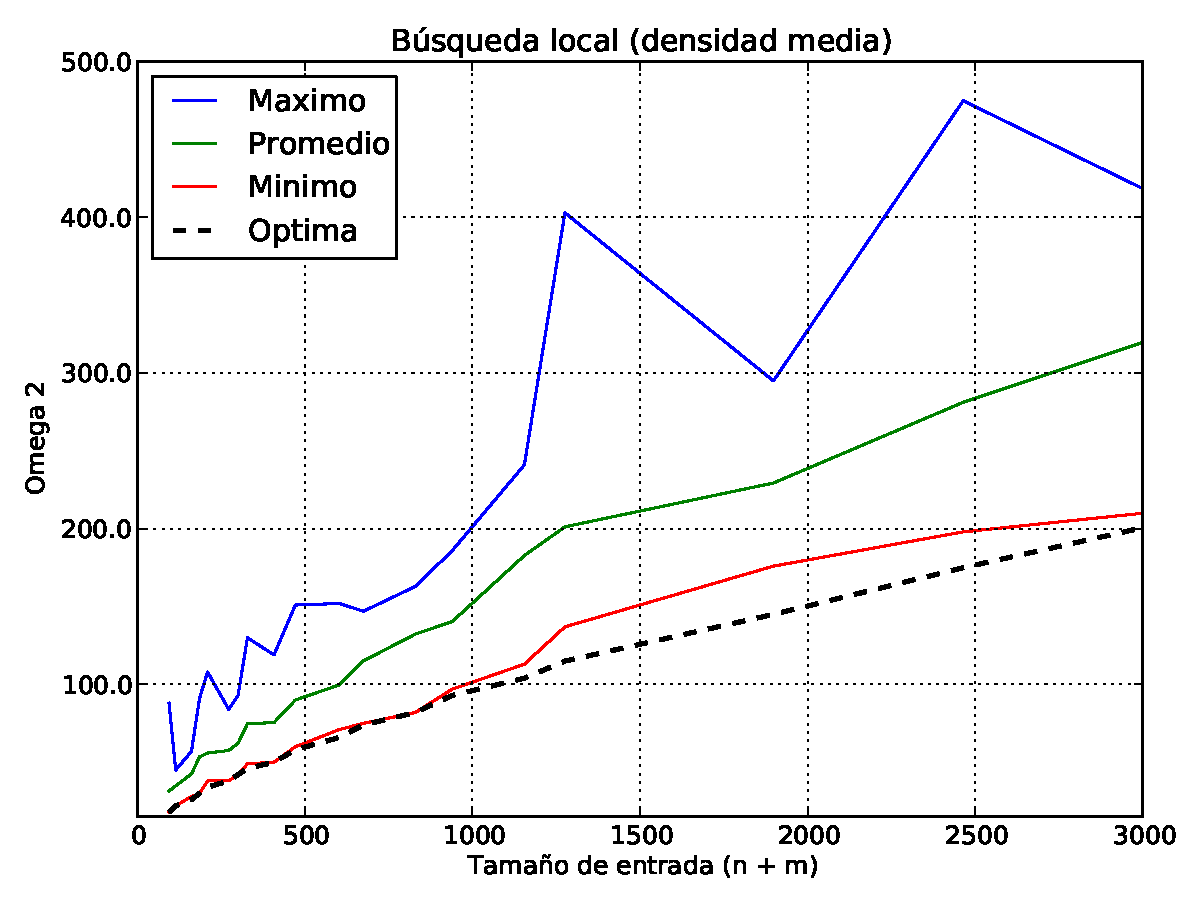
\includegraphics[angle=0, scale=.70]{imagenes/calidad_local_search_2014-06-27_08-58-52.pdf}
\label{grafico local}
\end{center}
\end{figure}

\begin{figure}[H]
\begin{center}
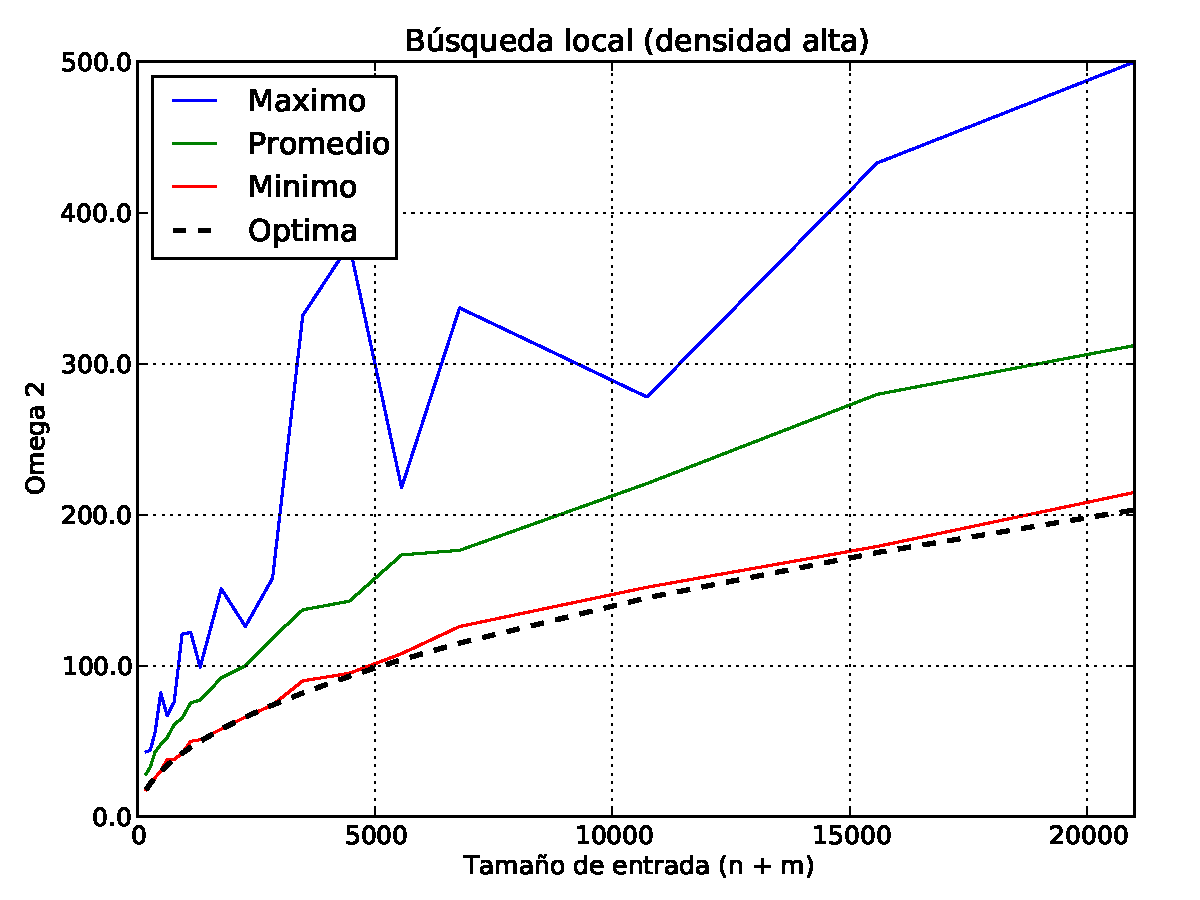
\includegraphics[angle=0, scale=.75]{imagenes/calidad_local_search_2014-06-27_08-54-45.pdf}
\label{grafico local}
\end{center}
\end{figure}

En los tres gráficos se puede notar, a medida que aumenta el tamaño de la entrada, una mayor amplitud de resultados. Ésto tiene cierta intuición. 
Se generan muchas instancias para cada tamaño. A medida que aumenta la cantidad de aristas y vértices, aumenta la variedad entre las instancias
generadas. Esto permite ver una gran diferencia de resultado entre instancias del mismo tamaño.
La solución media, no obstante, parece preservar cierta distancia relativa, cierta escala con respecto a la solución óptima.

La mejor solución encontrada siempre está muy cerca de la solución óptima. Ésto se evidencia particularmente en el tercer gráfico, lo que
atribuímos a la mayor densidad que le permite al algoritmo tener una vecindad amplia para recorrer. Sin embargo pareciera que la densidad también aumenta la amplitud y por lo tanto empeora la solución máxima. Puede tener sentido si se considera que al aumentar la cantidad de aristas que se deben generar cada una con su par de nodos y pesos, la diferencia entre dos instancias es combinatoria teniendo en cuenta todas las elecciones posbibles para cada arista.

A continuación se procede a estudiar la cantidad de iteraciones efectuadas por la búsqueda local, en relación a la cantidad de nodos del grafo.

\begin{figure}[H]
\begin{center}
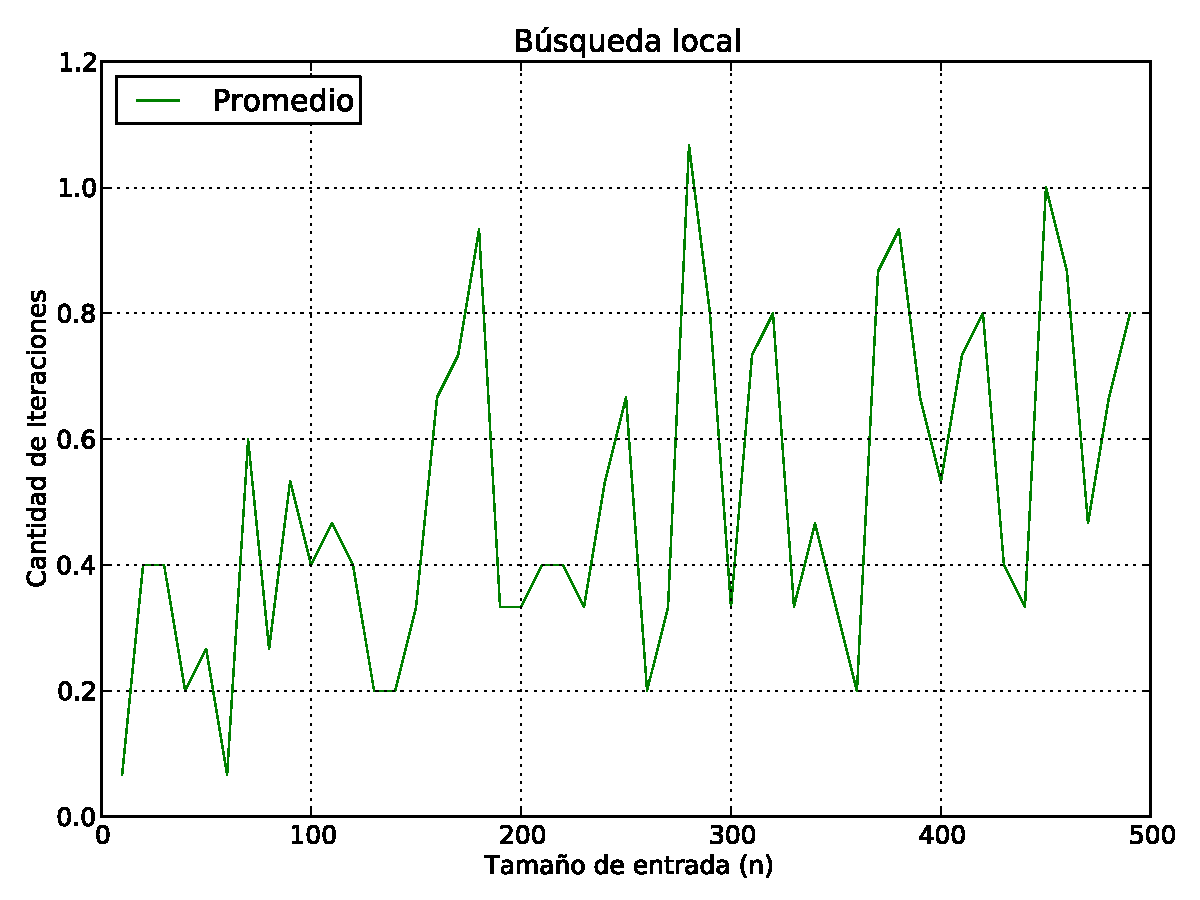
\includegraphics[angle=0, scale=.70]{imagenes/local-iteraciones.pdf}
\label{grafico local}
\caption{Cantidad de iteraciones en instancias \textit{mágicas}, de densidad media}
\end{center}
\end{figure}

La cantidad de iteraciones realizadas presenta una gran amplitud, aún para tamaños de grafo similares. Tiene sentido si se considera que diferentes adyacencias de nodos, aún cuando la cantidad de nodos y aristas es la misma, puede permitir o no a la búsqueda local elegir una mejor solución vecina. La cantidad de iteraciones muestra una tendencia lineal a crecer. Sin embargo se considera que es un resultado más bajo de lo esperado, ya  parte importante de una heurística de búsqueda local es que la solución tenga movilidad suficiente y no quedarse estático cerca de la solución inicial. Se notó una gran cantidad de casos en los que la búsqueda local no pudo mejorar la solución inicial.

Nos propusimos mejorar la perspectiva de la búsqueda local implementada, analizando la cantidad de unidades de $\omega_2$ que se disminuyen en cada iteración de la búsqueda local. 

\begin{figure}[H]
\begin{center}
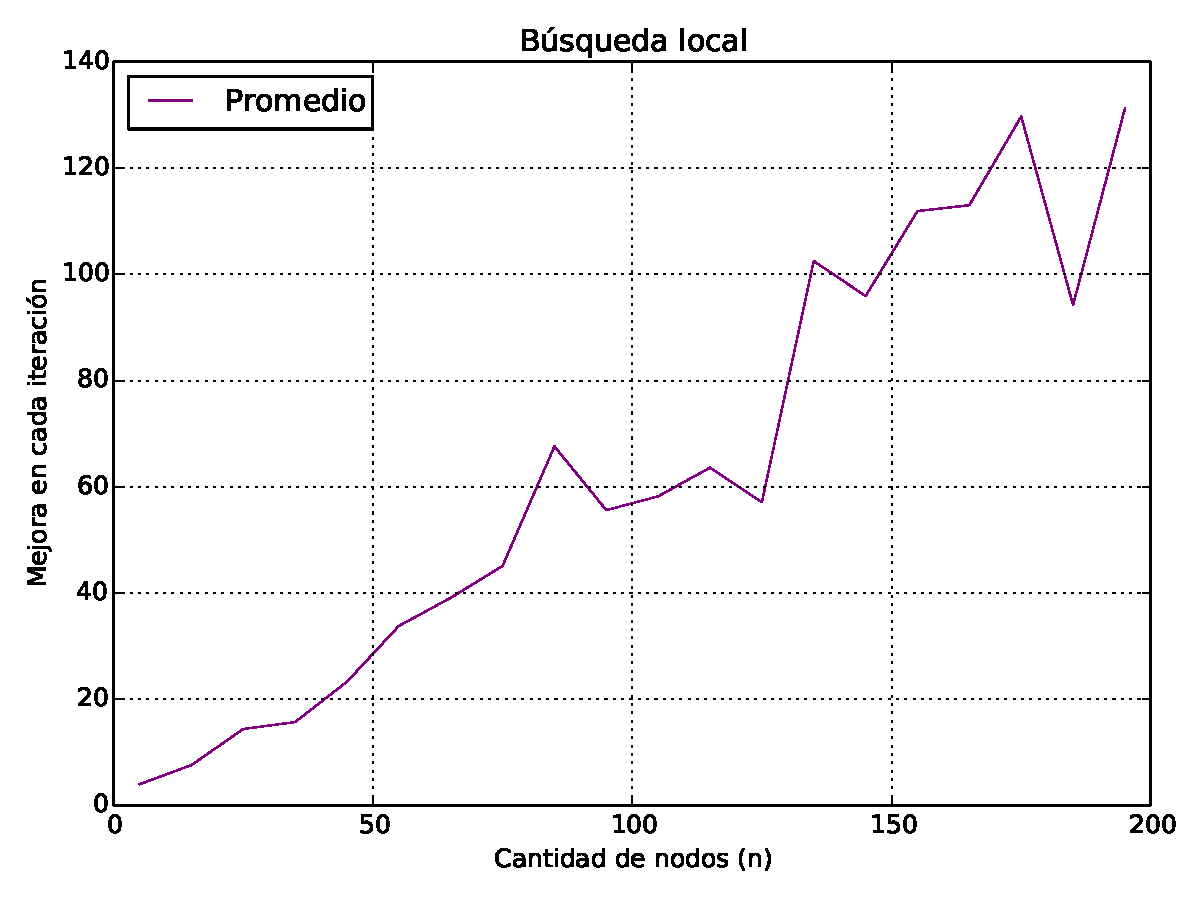
\includegraphics[angle=0, scale=.70]{imagenes/local_search-mejora.pdf}
\label{grafico local}
\caption{Mejora en cada iteración en instancias \textit{mágicas} de densidad media}
\end{center}
\end{figure}

Los resultados fueron sorprendentes. Como quedo expuesto anteriormente, una corrida de búsqueda local no suele hacer muchas iteraciones, pero cuando las hace, disminuye notablemente el valor de $\omega_2$ de la solución. Debe tenerse en cuenta que, siendo éstas instancias de tipo \textit{mágico}, el valor de $\omega_2$ de la solución óptima es $n-1$. De modo que lo que se ve en el gráfico es que el promedio de mejora en una iteración es del 60\% del valor de la solución óptima, proporción que se mantiene en las magnitudes de grafos consideradas.

